\section{Paired Testing}
\begin{frame}
  \begin{center}
  {\bf Part II -- Paired Testing}
  \end{center}
\end{frame}

\begin{frame}{Paired Comparison of Two Samples}{Outline}

  In the last part, we studied how to apply the statistical inference method using hypothesis testing to the situation where we want to compare two samples.\bigskip

  In this part, we will study a common special situation, where there is a strong dependency between observations in the samples.\bigskip

  The change in the calculation is very minor, but the results can be very different!
\end{frame}

\subsection{Motivation}
\begin{frame}{Examples of Paired Design}{Paired Design happens when the observations in both samples have strong dependencies.}

  \begin{block}{Example 1: Football shoes}
    Out of two brand of football shoes, you want to measure which one wears out faster.
    \begin{itemize}
      \item You make a team play two games, one with shoe A, one with shoe B. You measure the amount of wear for each player's shoes.
      \item You know that the Foward's shoes will wear much more than the Goalkeeper's shoes.
    \end{itemize}
  \end{block}
  \begin{block}{Example 2: Fuel Efficiency}
    You want to measure if a new kind of fuel is more efficient than an old one.
    \begin{itemize}
      \item You choose 10 cars, fill then with each type of fuel, make then run until they are out of fuel, and measure the distance.
      \item You know that different car types consume fuel at very different rates.
    \end{itemize}
  \end{block}
\end{frame}

\begin{frame}{Computer Science Example}{Comparison of Two Optimization Methods}

A researcher develops a new optimization algorithm (A), and wants to compare its
convergence speed against a method that represents the state-of-art (B).\bigskip

The researcher believes that the proposed algorithm has a theoretical advantage on a {\bf specific family of optimization problems}, so she selects a set of benchmark problems from that family.\bigskip

Both methods are executed on the benchmark set, and the time-to-convergence is measured for each problem. The measurements are made under homogeneous conditions (same computer, same operating conditions, etc).
\end{frame}

\begin{frame}{Computer Science Example}{Consideration for Experiment Design}

In this example, we are taking several problem instances, and running each
of the two algorithms in all instances. Because of the expected variation in
running time, we might want to run one "algorithm-instance" multiple times.\bigskip

This problem has some important questions worth considering:
\bigskip

\begin{itemize}
  \item What is the \structure{estimator} that should be measured in this experiment?
  \item What is one \structure{independent observation} for this experiment?
  \item What is the relevant sample size for the experiment?
\end{itemize}
\bigskip

\begin{block}{}
  Think about the difference between considering \structure{individual runs} as observations and \structure{individual problems} as observations.
\end{block}
\end{frame}


\subsection{Definitions}
\begin{frame}{Paired Experimental Design}{Why is Pairing Necessary?}

  When we consider observations with strong dependencies (players, cars types, benchmark problems), the difference between the observations is a strong source of variation (noise) that is not related to the objective of the experiment.\bigskip

  This variation can, and must, be controlled in the experiment design.\bigskip

  An elegant solution to eliminate the influence of this nuisance parameter is the \textit{pairing} of the measurements by problem:\bigskip

  \begin{itemize}
  \item Observations are considered in pairs (A, B) for each benchmark problem;
  \item Hypothesis testing is done on the sample of ""\textit{differences for a benchmark}";
  \end{itemize}
\end{frame}

\begin{frame}{Paired Experimental Design}{Statistical Model}
Let $y_{Aj}$ and $y_{Bj}$ be the paired observations of the average time for methods A and B, for a problem instance $j$. The \textit{paired difference} of an observation is simply $d_j = y_{Aj} - y_{Bj}$.
\bigskip

If we model our observations as an additive process:
\begin{equation*}
y_{ij} = \underbrace{\mu + \tau_i}_{\mu_i} + \beta_j + \varepsilon_{ij}
\end{equation*}
\noindent where $\mu$ is the grand mean, $\tau_i$ is the effect of the $i$-th method on the mean (A or B), $\beta_j$ is the effect of the $j$-th problem, and $\varepsilon_{ij}$ is the model residual, then:
\begin{equation*}
\begin{split}
d_j &= y_{Aj} - y_{Bj}\\
&= \mu + \tau_A + \beta_j + \varepsilon_{Aj} - (\mu + \tau_B + \beta_j + \varepsilon_{Bj})\\
&= \cancel{\left(\mu +\beta_j - \mu - \beta_j\right)} + \tau_A-\tau_B + \varepsilon_{Aj}-\varepsilon_{Bj}\\
&=\mu_{D} + \varepsilon_j\\
\end{split}
\end{equation*}

\end{frame}

\begin{frame}{Paired Experimental Design}{Hypotheses}
The hypotheses of interest can now be defined in terms of $\mu_D$, e.g.:
\begin{equation*}\begin{cases}
H_0: \mu_D = 0\\
H_1: \mu_D \neq 0
\end{cases}\end{equation*}

And now, we are back to our traditional "single sample hypothesis test". The population of interest is the difference in convergence time for the family of problems under investigation. The test statistic is given by:
\begin{equation*}
  T_0 = \frac{\bar{D}}{S_D/\sqrt{N}}\sim t^{(N-1)}
\end{equation*}
\bigskip

Where $\bar{D}$ is the average of the paired differences, and $N$ is the number of benchmark problems in the experiment.
\end{frame}


\begin{frame}{Paired Experimental Design}{Other Considerations}
Some other important questions worth considering:
\medskip

\begin{itemize}
\item In this example the minimally interesting effect size $\delta^*$ must be expressed in terms of \textit{average time gains across problems} (not within individual instances).
\item The most important sample size to consider in this situation refers to the \textit{number of problem instances}, and not necessarily to the number of within-problems repeated measures;
\item The number of repetitions within each problem will have an impact on the uncertainty associated to each observation (that is, to each value of mean time to convergence for each algorithm on each problem), which will propagate down to the residual variance.
\end{itemize}
\end{frame}



\begin{frame}{Paired Experimental Design}{Summary}

\begin{itemize}
  \item The Paired Design removes the effects of \structure{controllable} nuisance factors from the analysis. (Problem type, personal characteristics, etc)\bigskip

  \item It is strongly indicated in cases with {\bf strong correlations between samples}\\
  (e.g., heterogeneous experimental conditions).
\end{itemize}
\end{frame}

\subsection{Benchmark testing Example}

\begin{frame}{Paired Comparison Example}
Going back to our example, assume the following facts about the desired comparison:\bigskip

\begin{itemize}
\item The benchmark set is composed of seven problem instances ($N=7$);
\item The researcher is interested in finding differences in mean time to convergence greater than ten seconds ($\delta^*=10$) with a power of at least $(1-\beta)=0.8$, using a significance level $\alpha=0.05$;
\item The researcher performs $n=30$ repeated runs\footnote[1]{\tiny Not that this number is necessarily good, but it is generally an easy alternative if you don't want to keep justifying your choices to less statistically-savvy reviewers.} of each algorithm in each problem, from random initial conditions.
\end{itemize}
\end{frame}


\begin{frame}[fragile]{Executing the Paired Analysis}
  {Step 1: load and precondition the data}

\begin{columns}
  \column{0.7\textwidth}
{\smaller{\smaller
\begin{verbatim}
> # Read data from CSV file
> data <- read.table("benchmark.csv", header=T)

# Change the type of the "Problem" variable
#                 from "number" to "Factor"
> data$Problem <- as.factor(data$Problem)

# Summarize within-problem observations by mean
> aggdata <- aggregate(Time ~ Problem:Algorithm,
+                      data = data, FUN  = mean)
> summary(aggdata)
 Problem Algorithm      Time
 1:2     A:7       Min.   : 37.63
 2:2     B:7       1st Qu.:109.45
 3:2               Median :178.73
 4:2               Mean   :175.48
 5:2               3rd Qu.:245.25
 6:2               Max.   :296.79
 7:2
\end{verbatim}}}
\column{0.3\textwidth}
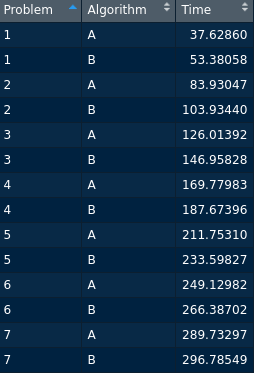
\includegraphics[width=1\textwidth]{../img/steelrods_summarytable}
\end{columns}
\end{frame}

\begin{frame}{Executing the Paired Analysis}{Influence of the problem type in the results}
      Note that the difference between problems is bigger than the difference between methods.
  \begin{center}

  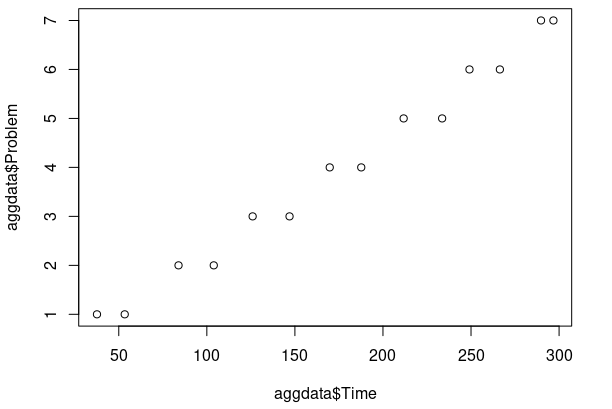
\includegraphics[width=.6\textwidth]{../img/steelrods_timediff}
  \end{center}
\end{frame}

\begin{frame}[fragile]{Executing the Paired Analysis}{Step 2: analysis}
  {\smaller
\begin{verbatim}
> # Perform paired t-test
> t.test(Time ~ Algorithm, data = aggdata,
+        paired = TRUE)           #  <-- To do a paired test, just change here.

Paired t-test
data:  Time by Algorithm
t = -9.1585, df = 6, p-value = 9.54e-05
alternative hypothesis: true difference in means is not equal to 0
95 percent confidence interval:
 -21.85862 -12.64118
sample estimates:
mean of the differences
               -17.2499
\end{verbatim}}
\end{frame}



%=====

\begin{frame}[fragile]
{Executing the Paired Analysis}
{Step 2: Alternate calculation}

{\smaller
\begin{verbatim}
# Create an array with the difference per problem, and perform one-sample test.
> difTimes <- aggdata$Time[1:7] - aggdata$Time[8:14])
> t.test(difTimes)

One Sample t-test
data:  difTimes
t = -9.1585, df = 6, p-value = 9.54e-05
alternative hypothesis: true mean is not equal to 0
95 percent confidence interval:
 -21.85862 -12.64118             # Same result!
sample estimates:
mean of x
 -17.2499
\end{verbatim}}
\bigskip

{\bf Check your understanding:} Why is the paired test on two samples equivalent to the one sample test on the difference vector of the samples?
\end{frame}

\begin{frame}[fragile]{Paired Analysis}{Step 3: Testing the assumptions}
  As usual, you should test the normality and variance of your data, and guarantee the independence of the observations. Let's check the normality test.
  \begin{columns}
    \column{0.6\textwidth}
{\smaller{\smaller
\begin{verbatim}
> shapiro.test(difTimes)
Shapiro-Wilk normality test
data:  difTimes
W = 0.8387, p-value = 0.09655

# Redo test without outlier
> indx <- which(difTimes == max(difTimes))
> t.test(difTimes[-indx])$p.value
[1] 6.179743e-06
> t.test(difTimes[-indx])$conf.int
[1] -21.41856 -16.48037
\end{verbatim}}}
\column{0.35\textwidth}
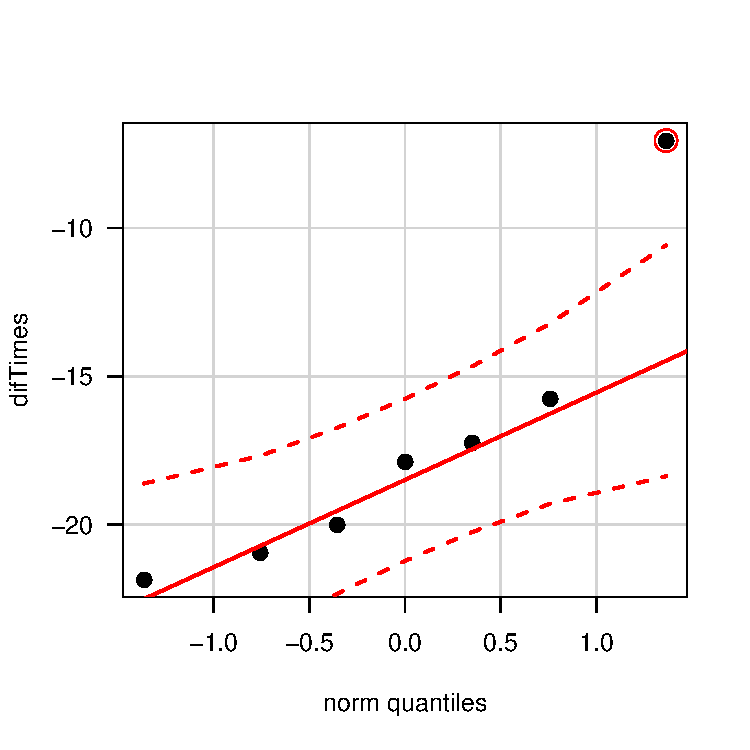
\includegraphics[width=.8\textwidth]{../img/soltimesqq.pdf}
\end{columns}
The normality test showed one big outlier. It does not invalidate the test, but
it should be examined. You might learn something important!
\end{frame}



%=====

\begin{frame}[fragile]{Why is Pairing Important?}{What happens if we ignore the dependency between observations?}
{\smaller
\begin{verbatim}
> t.test(Time ~ Algorithm, data = aggdata)

Welch Two Sample t-test
data:  Time by Algorithm
t = -0.3609, df = 11.993, p-value = 0.7245
alternative hypothesis: true difference in means is not equal to 0
95 percent confidence interval:
 -121.40320   86.90341
sample estimates:
mean in group A mean in group B
       166.8527        184.1026
\end{verbatim}}

If we don't take into account the large variation among problems, {\bf it will hide
variation between the two methods.}

% In a similar way, if we fail to recognize the similarity between observations, it is possible to artificially inflate $\alpha$ by \alert{pseudo-replication}.
\end{frame}

\begin{frame}{Why is Pairing Important?}{A visual Comparison}
  \begin{columns}
    \column{0.5\textwidth}
    \begin{center}
      Paired Samples
    \end{center}
    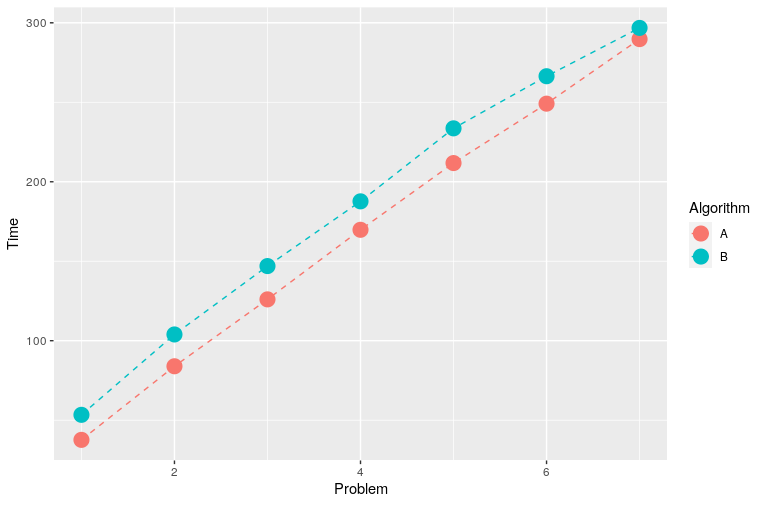
\includegraphics[width=\textwidth]{../img/2samples_paired}
    \column{0.5\textwidth}
      \begin{center}
        Unpaired Samples
      \end{center}
    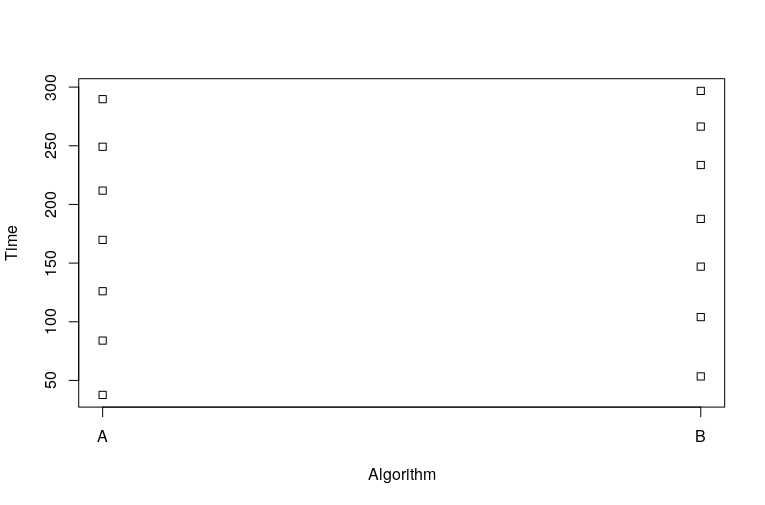
\includegraphics[width=\textwidth]{../img/2samples_unpaired}
  \end{columns}
\end{frame}

%=====
%
% \begin{ftstf}
% {Comparison of two means}
% {Paired design}
% Paired designs can require smaller sample sizes for equivalent power in cases where the between-units (in our example, the between-problems) variation is relatively high;
% \vhalf
% More specifically, if the within-level variation is given by $\sigma_\epsilon$ and the between-units variation is $\sigma_u$, we have that, for large enough $N$\\(e.g., $N\geq 10$),
% \beqs
% \frac{N_{\mbox{\tiny unpaired}}}{N_{\mbox{\tiny paired}}}\approx\sqrt{2\left[\left(\frac{\sigma_u}{\sigma_\epsilon}\right)^2+1\right]}
% \eqs
% \vhalf
% Failure to consider inter-unit variability can result in the masking of relevant effects by the nuisance factor.
% \vhalf
% Similarly, failure in recognizing the dependence structure of within-unit measurements yields tests with artificially inflated degrees of freedom, which results in the inflation of the effective value of $\alpha$.
% \end{ftstf}

%% My slide: A few more examples of paired testing.
